\documentclass{trlnotes}
\setlayout{hardcopy}
\usepackage{silence}
\WarningFilter{latex}{Reference}
\graphicspath{{../../img/}}

\begin{document}
    \paragraph{Разностный метод для общего уравнения теплопроводности, явная схема}

    \begin{de}
        Общее \ti{уравнение теплопроводности} выглядит вот так:
        \[
            \dfrac{\pd u}{\pd t} = a_0 \dfrac{\pd^2 u}{\pd x^2} + a_1 \dfrac{\pd y}{\pd x} + a_2 u + f.
        \]
        Функции $a_i$ и $f$ зависят от $x$ и $t$.
    \end{de}

    Работать будем, как всегда, на отрезке $[a, \, b]$; временной отрезок будет $[0, \, T]$.

    \begin{de}
        У уравнения теплопроводности бывает \ti{начальное условие}:
        \[
            u(x, \, 0) = \varphi(x),            
        \]
        а также три типа \ti{граничных условий}
        \begin{enumerate}
            \item $u(a, \, t) = \psi_0(t)$, $u(b, \, t) = \psi_1(t)$.
            \item $\dfrac{\pd u}{\pd x}(a, \, t) = \psi_0(t)$, $\dfrac{\pd u}{\pd x}(b, \, t) = \psi_1(t)$.
            \item $\dfrac{\pd u}{\pd x} - \alpha u \big|_{x = a} = \psi_0(t)$, $\dfrac{\pd u}{\pd x} - \beta u \big|_{x = b} = \psi_1(t)$.
        \end{enumerate}
    \end{de}
    Сетка характеризуется такими же, как обычно, величинами:
    \[
        \begin{array}{lll}
            x_i = a + ih, & h = \dfrac{b - a}{h}, & i \in 0\ldots n; \\
            t_k = k\tau, & \tau = \dfrac{T}{M}, & k \in 0 \ldots M.
        \end{array}
    \]

    Положим $u_i^k = u(x_i, \, t_k)$ и
    \[
        Lu = a_0 \dfrac{\pd^2 u}{\pd x^2} + a_1 \dfrac{\pd y}{\pd x} + a_2 u.
    \]
    Тогда
    \[
        (\tilde{L}u)_i^k = a_0 \dfrac{u_{i+1}^k - 2u_i^k + u_{i - 1}^k}{h^2} + a_1 \dfrac{u_{i + 1}^k - u_{i - 1}^k}{2h} + a_2 u_i^k.
    \]
    Есть два варианта для производной по времени:
    \begin{align}\label{eq:therm-A-B}
        &\text{A:} \quad \dfrac{\pd u}{\pd t}(x_i, \, t_k) \approx \dfrac{u^{k + 1}_i - u^k_i}{\tau}, \\
        &\text{B:} \quad \dfrac{\pd u}{\pd t}(x_i, \, t_k) \approx \dfrac{u^{k}_i - u^{k-1}_i}{\tau}.
    \end{align}
    Для варианта A получается 
    \[
        \boxed{\dfrac{u_i^{k + 1} - u_i^k}{\tau} = \tilde{L}u_i^k + f(x_i, \, t_k)}\,.
    \]
    Это простейшая явная схема. 

    \begin{figure}[h] \label{fig:therm-simple}
        \begin{center}
            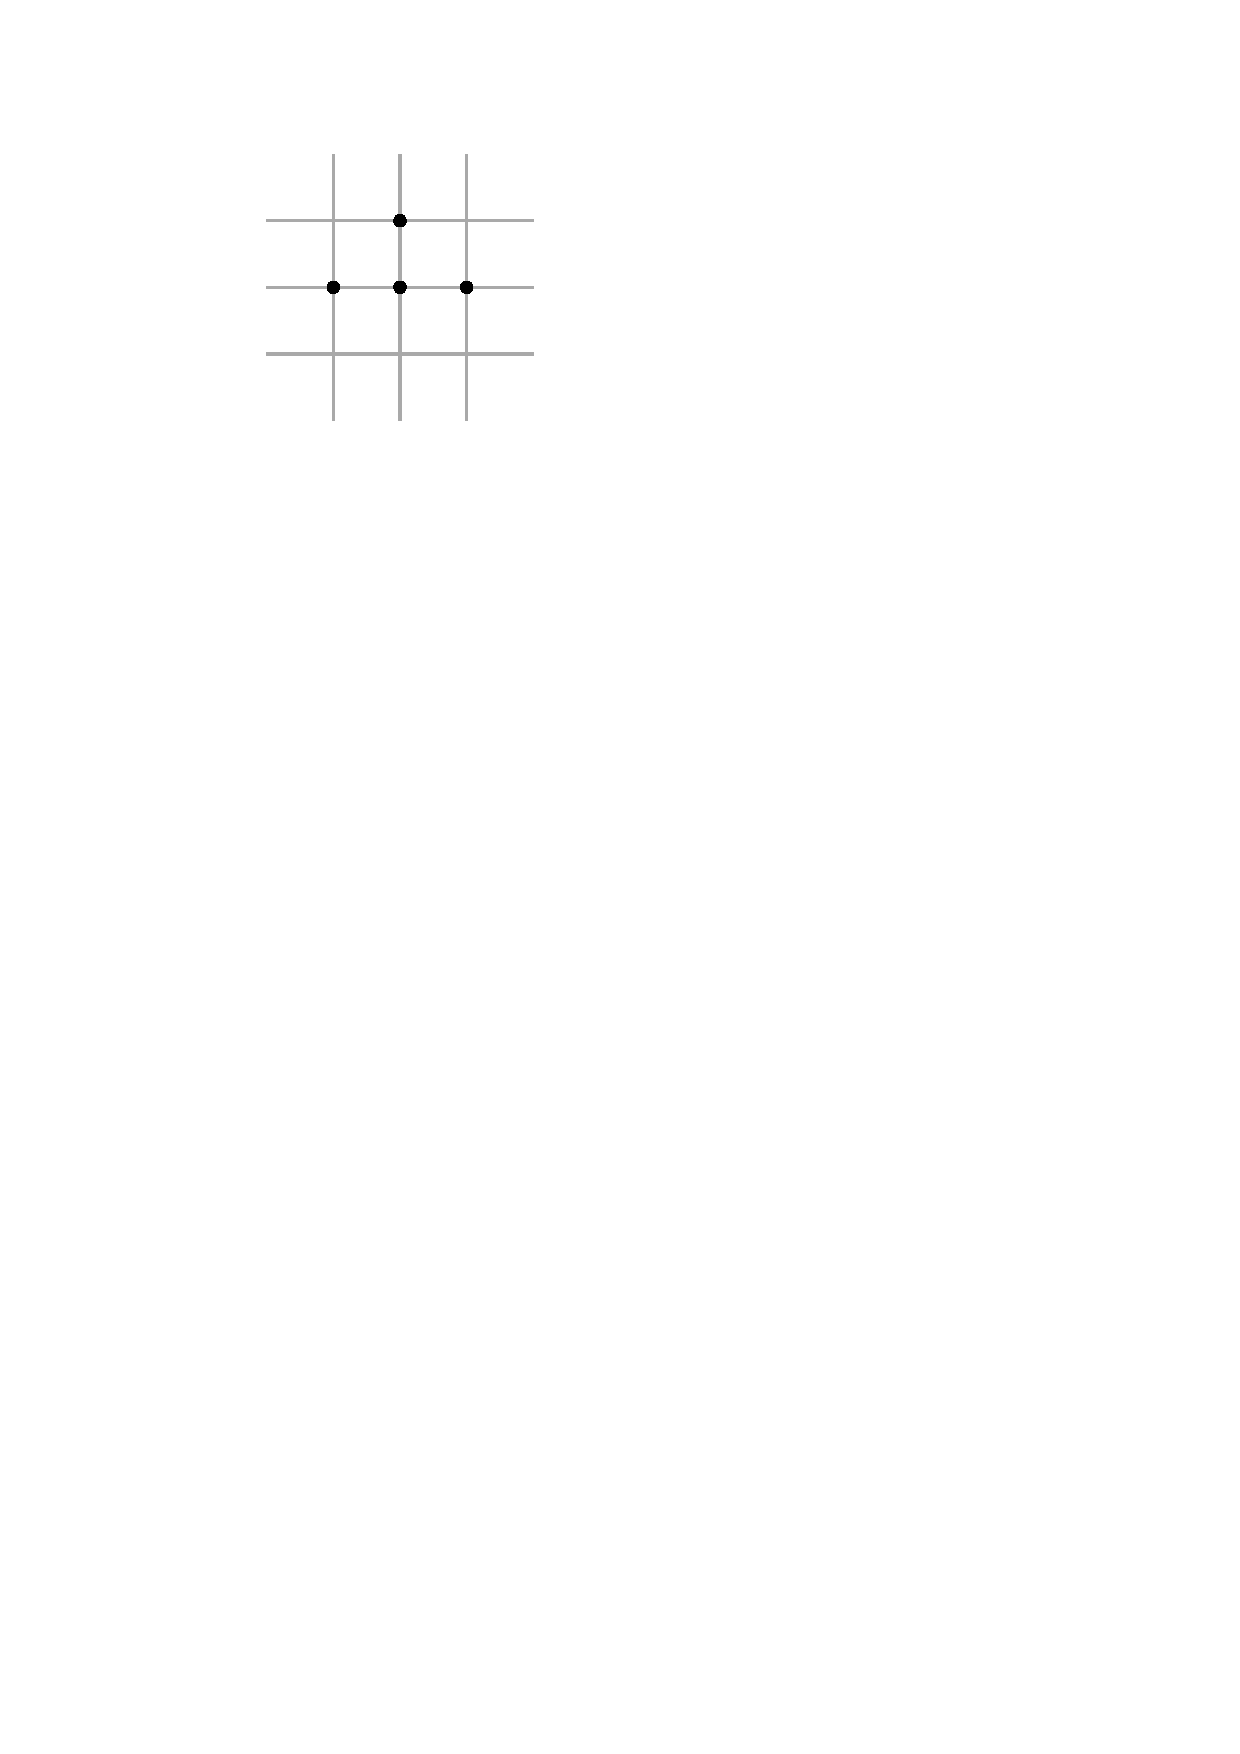
\includegraphics[scale=0.9]{../img/pde/therm-simple.pdf}
        \end{center}
        \caption{Простейшая явная схема для уравнения теплопроводности.}
    \end{figure}

    В таком виде уравнения можно писать для $i \in 1\ldots n-1$, $k\in 0\ldots M-1$; нужны дополнительные с граничными условиями. 

    \begin{itemize}
        \item Начальные условия: $u_i^0 = \varphi(x_i)$.
        \item Граничные условия:
        \begin{enumerate}
            \item $u_0^k = \alpha_1(t_k)$, $u_n^k = \alpha_2(t_k)$; при этом выполняются условия согласования \ti{нулевого порядка}
            \[
                \varphi(a) = \alpha_1(0), \quad \varphi(b) = \alpha_2(0).
            \]
            \item Для типов II, III используются такие же трюки, как в обычных диффурах. Надо аппроксимировать производные. Можно применять метод фиктивных точек или метод исключения главного члена погрешности.

            В угловых точках снова возникнет два разных условия:
            \[
                u_0^0 = \varphi(a) \text{ и } \dfrac{\pd u}{\pd x}(a, \, 0) = \beta_1(0) u_0^0 + \alpha_1(0).
            \]
            Будет ли выполняться равенство
            \[
                \varphi'(a) = \beta_1(0) u_0^0 + \alpha_1(0)?
            \]
            Оно называется \ti{условием согласования I порядка}. Без него уравнения не станут формально противоречивы.
        \end{enumerate}
    \end{itemize}

    Если разрешить уравнения относительно $u_i^{k + 1}$, получится 
    \[
        u_{i}^{k + 1} = A_i^k u_{i-1}^k + B_i^k u_i^k + C_i^k u_{i+1}^k + D_i^k.
    \]
    Коэффициенты выражаются по формулам
    \[
        \begin{array}{ll}
            A_i^k = \sigma a_0 - \sigma a_1 \dfrac{h}{2}, & C_i^k = \sigma a_0 + \sigma \dfrac{h}{2} a_1, \\
            B_i^k = 1 - 2 \sigma a_0 + \tau a_2,  &D_i^k = \tau f(x_i, \, t_k),
        \end{array}
    \]
    где $\sigma = \dfrac{\tau}{h^2}$.

    Можно просто двигаться вперёд по \ti{слоям}~--- множествам точек с постоянным временем; значения находятся последовательно.

    \paragraph{Неявная схема для уравнения теплопроводности}

    Неявная схема получается, если в \ref{eq:therm-A-B} выбрать вариант B. Сверху вниз (т.е. назад по времени) просчитать не получится, поскольку начальные данные даются в начале, а не в конце.

    \begin{figure}[h] \label{fig:therm-implicit}
        \begin{center}
            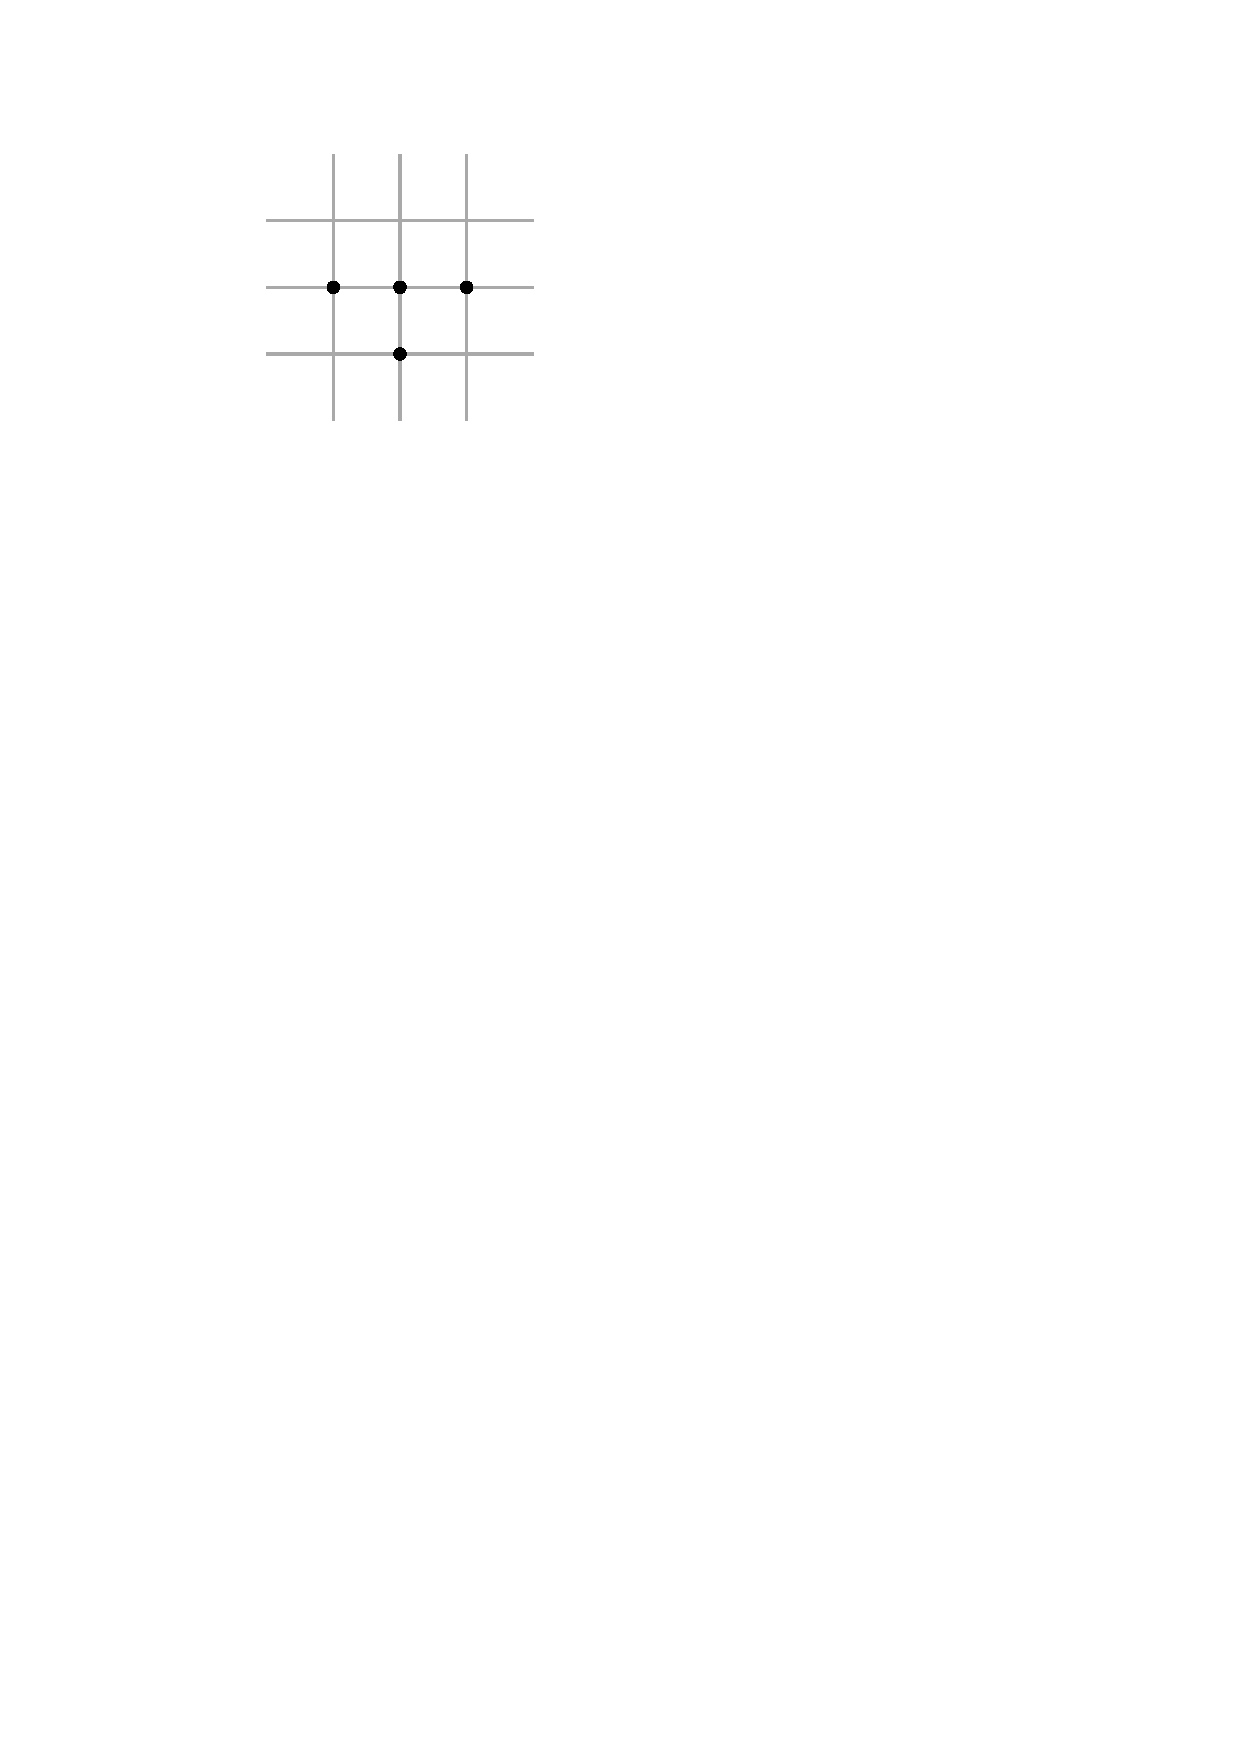
\includegraphics[scale=0.9]{../img/pde/therm-implicit.pdf}
        \end{center}
        \caption{Неявная схема для уравнения теплопроводности.}
    \end{figure}

    Формулы получатся такие:
    \[
        A_i^k u_{i-1}^k - B_i^k u_i^k + C_i^k u_{i+1}^k = D_i^k,
    \]
    где
    \[
        \begin{array}{ll}
            A_i^k = \sigma a_0 - \sigma a_1 \dfrac{h}{2}, & C_i^k = \sigma a_0 + \sigma \dfrac{h}{2} a_1, \\
            B_i^k = 1 + 2 \sigma a_0 - \tau a_2,  &D_i^k = -u_i^{k-1} - \tau f(x_i, \, t_k),
        \end{array}
    \]
    и $\sigma = \dfrac{\tau}{h^2}$.

    По сути, движение всё ещё послойное. Но на каждом слое я не могу просто посчитать значение, используя три значения с предыдущего слоя: наоборот, получается уравнение, которое связывает три значения с текущего слоя с одним уже известным. В итоге получается система с трёхдиагональной матрицей, которая замыкается добавлением граничных условий:
    \[
        u_0^k = \alpha_1(t_k), \; u_n^k = \alpha_2(t_k),
    \]
    если они заданы по первому типу, в противном случае применяются стандартные аппроксимации. 

    Система решается методом разностной прогонки \ref{par:ode::fintdma}.

    %unsure
    Кажется, тут утверждается, что метод прогонки срабатывает, поскольку
    \[
        A_i^k + C_i^k = 2\sigma a_0 = B_i^k + \tau a_2 - 1,
    \]
    и можно сослаться на \ref{prop:ode::diffeqest::suff}. Наверное, на практике это правда так, потому что $\tau a_2 \ll 1$, но выглядит сомнительно, я чего-то не понял.
    %unsure

    \paragraph{Явная схема для простейшего уравнения теплопроводности, решение разностных уравнений, неустойчивость}

    Рассмотрим уравнение
    \[
        \dfrac{\pd u}{\pd t} = \dfrac{\pd^2 u}{\pd t^2}, \quad t \in [0, \, \pi].
    \]
    с начальным условием $u(x, \, 0) = \varphi(x)$ и граничными условиями
    \[
        u(0, \, t) = u(\pi, \, t) = 0
    \]

    Для него разностные уравнения исключительно просты:
    \[
        \dfrac{u^{k + 1}_l - u^k_l}{\tau} = \dfrac{u^k_{l + 1} - 2u^k_l + u^k_{l-1}}{h^2}, \quad u_0^k = u_n^k = 0.
    \]
    При этом
    \[
        h = \dfrac{\pi}{n}, \quad x_l = lh, \quad u_l^0 = \varphi(x_l).
    \]

    Решим наше разностное уравнение методом разделения переменных, будем искать решение в виде
    \[
        u_l^k = \lambda^k e^{imx}, \quad x = x_l = lh.
    \]
    Подставим:
    \[
        \dfrac{\lambda^{k + 1}e^{imx} - \lambda^{k}e^{imx}}{\tau} = \dfrac{\lambda^k e^{im(x+h)} - 2\lambda^k e^{imx} + \lambda^k e^{im(x-h)}}{h^2}.
    \]
    Несложными выкладками отсюда находится
    \[
        \lambda = 1 + 2\sigma \big(\cos mh - 1\big)\,, \quad \sigma = \dfrac{\tau}{h^2}.
    \]
    Но такое решение не удовлетворяет граничным условиям; можно рассмотреть какую-нибудь комбинацию решений! Заметим, что $\lambda(m)$~--- чётная функция, поэтому 
    \[
        \lambda^k(m) \big(e^{imx} - e^{-imx}\big) = 2i\lambda^k(m)\sin(mx)
    \]
    тоже решение. Оно удовлетворяет граничным условиям при целых $m$; в итоге получаем
    \[
        \boxed{u_l^k = \lambda^k(m) \cdot \sin (mx), \quad m \in \Z}\,.
    \]
    У нас теперь есть $n-1$ ЛНЗ решение, из которых можно собирать новые:
    \[
        \varphi(x) = \sum\limits_{m = 1}^{n - 1} C_m \lambda^k(m) \cdot \sin (mx).
    \]

    \begin{rem}
        Остальные значения $m$ нам не интересны, поскольку у нас набралась $n-1$ базисная функция: действительно, изначально наши разностные уравнения решались однозначно, а сейчас мы их решили, учитывая граничные условия, но отпустив начальные. А их как раз $n - 1$~--- от $u^0_1$ до $u^0_{n-1}$, они и создают все степени свободы.
    \end{rem}

    Рассмотрим $\tau = h^2 \so \sigma = 1$:
    \[
        \lambda(m) = -1 + 2 \cos mh.
    \]
    При $m = n - 1$ и густой сетке (большом $n$)
    \[
        \cos \dfrac{(n - 1)\pi}{n} = \cos \left(\pi - \dfrac{\pi}{n}\right) \approx -1 \so \lambda(n - 1) \approx -3!
    \]

    При увеличении $k$ решение
    \[
        (-3)^k \sin(n - 1)x
    \]
    очень быстро растёт по модулю и всё время меняет знак. Кажется, что-то пошло не так!

    \begin{rem}
        Реальное решение такой задачи~--- быстро убывающая колебашка. Конечно, пространственный шаг взят большим: у начальных данных есть переменность на том же масштабе. Однако то, что при уменьшении шага по времени $k$ получает возможность становиться больше, уже вообще ни в какие ворота не лезет.
    \end{rem}

    %unsure
    %когда говорят про устойчивость, имеют в виду схему с фиксированным \tau или нет?
    %unsure

    Чтобы решения не вымирали подобным образом, можно наложить ограничение $|\lambda| \leqslant 1$:
    \[
        1 + 2\sigma \big(\cos mh - 1\big) \leqslant 1 \so 2\sigma \cos mh - 1 \leqslant 0 \so 2 \sigma \cos mh \leqslant 1.
    \]
    Чтобы это выполнялось при любых $m$, нужно, чтобы
    \[
        \boxed{\sigma \leqslant \dfrac{1}{2} \eqv \tau \leqslant \dfrac{h^2}{2}} \, .
    \]

    Если точно так же решить разделением переменных систему уравнений для простейшей неявной схемы, получим
    \[
        \lambda = \dfrac{1}{1 + 2\sigma(1 - \cos mh)} \leqslant 1,
    \]
    и устойчивость всегда присутствует.

    \paragraph{Общее определение устойчивости, теорема об устойчивости и сходимости}

    В начале книги \cite{gavurin} есть общие рассуждения про вычислительные методы и всякие пространства. В книге \cite{comp-krilov-2} есть про устойчивость, аппроксимацию, сходимость, их связь между собой, и про схемы для уравнения теплопроводности.

    С какой ситуацией мы сталкиваемся, занимаясь сеточными методами? У нас есть оператор $A\col \; U \to F$, и мы решаем уравнение вида
    \[
        Au = f.
    \]
    Выбирая сетку с шагом $h$ на отрезке, мы вместо функций на отрезке начинаем рассматривать функции на самой сетке~ они образуют другое, гораздо более маленькое пространство $U_h$. При этом по любому элементу $U$ можно легко найти элемент $U_h$, просто вычислив его значения на сетке. Аналогично строится пространство $F_h$\footnote{Зачастую $U_h = F_h$ и даже $U = F$, но может быть и не так, в принципе~--- вдруг, например, оператор действует в пространство функций на другом отрезке, или просто там другие ограничения на гладкость/непрерывность.}.

    Наконец, есть оператор $A_h \col \; U_h \to F_h$~--- приближение $A$, которое получается при переходе к конечным разностям. Для иллюстрации полезна диаграмма
    \[
        \xymatrix{
            U \ar@{->}[r]^{A} \ar@{->}[d]_{\varphi_h} & F \ar@{->}[d]^{\psi_h} \\ U_h \ar@{->}[r]^{A_h} & F_h
        }
    \]
    \begin{de}
        Операторы $\varphi_h(u)(x_l) = u(x_l)$ и такой же $\psi_h$ называются \ti{операторами (простого) сноса}.
    \end{de}

    \begin{rem}
        Понятно, что диаграмма должна быть почти коммутативна, но не совсем: если мы сначала продифференцируем функцию, а потом возьмём результат на сетке, и если мы сначала возьмём её на сетке, а потом посчитаем разностный аналог производной, получатся близкие, но разные вещи. Разность
        \[
            A_h\varphi_h(u) - \psi_h(Au)
        \]
         называется \ti{естественной погрешностью метода}.
    \end{rem}

    Далее, записывается разностное уравнение
    \[
        A_h \tilde{u} = \psi_h(f)
    \]
    и решается.

    Во всех четырёх пространствах надо ввести нормы. В пространствах функциональной природы $U$, $F$ они уже и так есть, вероятно.

    \begin{de}
        Говорят, что норма на $U_h$ \ti{согласована} с нормой на $U$, если верно, что 
        \[
            \|\varphi_h u\|_{U_h} \to \|u\|_U,
        \]
        когда $h \to 0$ хотя бы для $u \in K \subset U$, где $K$ плотно в $U$.

    \end{de}

    Будем считать, что у нас нормы согласованы.

    \begin{de}
        Говорят, что $A_h$ \ti{аппроксимирует} $A$ на $u \in U$, если 
        \[
            \big\|A_h\varphi_h(u) - \psi_h(Au)\big\| \to 0 \text{ при } h \to 0.
        \]
    \end{de}

    \begin{de}
        Говорят, что сеточные функции $u_h$ сходятся к функции $u \in U$, если 
        \[
            \big\|u_h - \varphi_h(u)\big\| \to 0 \text{ при } h \to 0.
        \]
    \end{de}

    \begin{de}
        Говорят, что \ti{сеточное приближение} обладает \ti{свойством аппроксимации}, если $A_h$ аппроксимирует $A$, и сеточные функции $f_h$ сходятся к $f$.
    \end{de}

    \begin{de}  
        Говорят, что сеточное приближение \ti{устойчиво}, если
        \begin{enumerate}
            \item Уравнение $A_hu_h = f_h$ однозначно разрешимо для всех $f_h \in F_h$;
            \item Для этого решения $\|u_h\| \leqslant k \|f_h\|$, где $k$ не зависит от $h$.
        \end{enumerate}
    \end{de}

    \begin{thm}[Основная теорема теории разностных методов]
        Пусть дана некоторая краевая задача, и сеточная аппроксимация удовлетворяет следующим свойствам:
        \begin{enumerate}
            \item $u^*$~--- единственное решение уравнения $Lu^* = f$.
            \item Сеточное приближение обладает свойством аппроксимации.
            \item Сеточная задача устойчива.
        \end{enumerate}
        Тогда есть сходимость сеточных решений: $u^*_h \to u$.
        \begin{proof}
            Запишем ошибку сеточного решения:
            \[
                w_h = u_h^* - \varphi_h u^*.
            \]
            Заметим, что по свойству устойчивости
            \begin{align*}
                \|w_h\| &\leqslant k \|L_h w_h\| = k\|L_h u_h^* - L_h \varphi_h u^*\| = \\ &= k\|f_h - \psi_h f + \psi_h f - L_h \varphi_h u^*\| \leqslant k\|f_h - \psi_h f\| + k\|\psi_h L u^* - L_h \varphi_h u^*\|.
            \end{align*}
            Оба слагаемых в правой части стремятся к нулю по свойству аппроксимации.
        \end{proof}
    \end{thm}

    \paragraph{Разностные схемы для задач с начальными условиями, дискретное преобразование Фурье}

    \begin{rem}
        ПРОИЗОШЛО СЖАТИЕ С ПОТЕРЯМИ ШАКАЛОМЕТР ЗАШКАЛИВАЕТ БИП 
    \end{rem}

    В этом параграфе в целом посмотрим на уравнение 
    \[
        \dfrac{\pd u}{\pd t} = Lu + f,
    \]
    где всё многомерное (т.е. $u$~--- вектор, а $L$~--- <<матрица>> из частных производных), и $L$~--- линейный дифференциальный оператор с постоянными коэффициентами. Область определения $u$~--- цилиндр $D\times [0, \, T] \subset \R^{p + 1}$. Начальные условия~--- $u(x, \, 0) = \varphi(x)$.

    Ограничимся теперь ситуацией, когда $D$~--- куб $[0, \, 2\pi]^p$, а граничные условия периодические по каждой из переменных (т.е. $u(x_1, \ldots, \, 0, \ldots, \, x_p; \, t) = u(x_1, \ldots, \, 2\pi, \ldots, \, x_p; \, t)$). 

    По каждой из пространственных переменных выберем одинаковые шаги
    \[
        h = \dfrac{2\pi}{N},
    \] 
    а по временной~--- шаг
    \[
        \tau = \dfrac{T}{M}.
    \]
    По пространственной причём рассматриваем только от $0$ до $M-1$, потому что справа снова будет то же граничное значение. Уравнения будут двухслойными, с $k$-го и $k+1$-го слоя.

    Даже в неявном случае с помощью разностной прогонки можно выразить все следующие слои через предыдущие и получить уравнения
    \[
        u_h(k + 1) = R_h u_h(k) + \rho_h(k),
    \]
    где $R_h$~--- \ti{оператор перехода в однородном случае}. $R_h$~--- просто матрица с постоянными коэффициентами, а $\rho_h(k)$ зависит от $f$.

    \begin{rem}
        Всё-таки скажу про эти обозначения пространств... $V_h$~--- пространство сеточных функций \ti{на фиксированном слое} (т.е. оно $N$-мерное), а $F_h$~--- видимо, аналогичное пространство, которое мы отличаем только по формальным причинам, в котором лежат $f_h$~--- сеточные версии $f$. Нормы в обоих пространствах~--- просто $l^{\infty}$, т.е.
        \[
            \big\|\{u_i\}\big\| = \max |u_i|.
        \]
    \end{rem}

    \begin{thm} \label{thm:stab-1}
        Для устойчивости при $f = 0$ необходимо и достаточно, чтобы были ограничены $\|R_h^k\|$ (здесь $k$~--- степень!) при $k\tau \leqslant T$.
        \begin{proof}
            Оно в целом понятно: когда нет $f$-ок, нет и $\rho$-шек, а без них переход на следующий слой~--- тупо умножение на матрицу $R_h$. Ясно, что если нормы этих матриц в совокупности ограничены, то и
            \[
                \|u_h(k+1)\| \leqslant C \|\varphi\|,
            \]
            где $\varphi$ задаёт начальные условия.

            Обратно тоже понятно: если ограниченности норм матриц нет, можно просто пойти от противного и сконструировать мерзкую последовательность.
        \end{proof}
    \end{thm}

    \begin{thm}
        Если $f \neq 0$ и $\|R_h^k\|$ ограничены, то для устойчивости достаточно, чтобы
        \[
            \|\rho_h\|_{V_h} \leqslant c_2 \tau \|f_h\|_{F_h}
        \]
        \begin{proof}
            Обычная оценка, см. конспект Ангелины, страница 75.
            %unsure
        \end{proof}
    \end{thm}

    \begin{cor}
        Если $\|R_h\| \leqslant 1 + c_3\tau$, то есть устойчивость (при $f = 0$).
        \begin{proof}
            \[
                \|R_h^k\| \leqslant \|R_h\|^k \leqslant (1 + c_3 \tau)^k \leqslant e^{c_3 \tau k} \leqslant e^{c_3 \tau}.
            \]
        \end{proof}
    \end{cor}

    По поводу этих теорем можно ещё заглянуть в следующий параграф \ref{par:neumann}, там доказаны очень похожие вещи.

    Перейдём теперь к дискретному преобразованию Фурье. Пусть размерность $p$ пока равна $1$. Введём на пространстве $V_h$ функций на фиксированном слое скалярное произведение:
    \[
        (u_h, \, v_h) = h \sum\limits_{i = 0}^{N - 1} u_h \ov{-}{v_h}
    \]

    \begin{st}
        Набор функций $e_m(x) = e^{imx}$, где $m \in 0\ldots N-1$, образует ортогональный базис в $V_h$, причём
        \[
            (e_m, \, e_m) = 2\pi.
        \]
        \begin{proof}
            Чтобы увидеть, что они ортогональны, достаточно посчитать скалярное произведение. Отсюда следует, в принципе, что они ЛНЗ. Ну а дальше~--- их $N$, пространство $N$-мерное, потому и базис.
        \end{proof}
    \end{st}

    \begin{de}
        \ti{Обратное дискретное преобразование Фурье}~---
        \[
            \{a_1, \, \ldots, \, a_N\} \mapsto \sum\limits_{i = 1}^{N-1} a_i e_i(x).
        \]
        \ti{Прямое ДПФ}~---
        \[
            u_h \mapsto \dfrac{1}{2\pi}\big\{(u_h, \, e_1), \ldots, \, (u_h, \, e_n)\big\}.
        \]
        Ясно, что это взаимно обратные операторы.
    \end{de}

    \begin{st}[Формула замкнутости]
        Дискретное преобразование Фурье~--- почти унитарный оператор, т.е. 
        \[
            \left(\sum\limits_{i = 1}^{N - 1} a_i e_i, \; \sum\limits_{i = 1}^{N - 1} b_i e_i\right) = 2 \pi \sum_{i = 0}^{N - 1} a_i \ov{-}{b_i}.
        \]
        \begin{proof}
            Проверяется прямым вычислением.
        \end{proof}
    \end{st}

    \begin{st}
        $e^{imx}$~--- собственная функция оператора сдвига
        \[
            T_h u(x) = u(x + h)
        \]
        с собственным числом $e^{imh}$.
        \begin{proof}
            Действительно,
            \[
                T_h e^{imx} = e^{im(x + h)} = e^{imh} e^{imx}.
            \]
        \end{proof}
    \end{st}

    \begin{rem}
        У нас периодические граничные условия, поэтому оператор сдвига может действовать, <<переходя>> через границу:
        \[
            T_h \{u_0, \, \ldots, \, u_{N - 1}\} = \{u_{1}, \, u_2, \, \ldots, \, u_{N-1}, \, u_0\}.
        \]
        Можно представлять себе, что индекс $i$ на самом деле меняется от $-\infty$ до $\infty$, но $u_{i + N} = u_i$. Периодическую функцию можно восстановить, зная её значения внутри периода, вот и здесь так же.
    \end{rem}

    \begin{rem}
        В такой ситуации любой разумный разностный оператор можно собрать из операторов сдвига. Например, пусть
        \[
            (Du)_i = \dfrac{u_{i + 1} - 2u_i + u_{i - 1}}{h}.
        \]
        Это можно переписать просто как
        \[
            Du = \dfrac{T_hu - 2u + T_{-h}u}{h}.
        \]
        Общая формула, естественно, будет такая:
        \[
            Lu = \sum\limits_{\alpha} c(\alpha) T_h^{\alpha}(u),
        \]
        где $\alpha \in \Z$~--- показатель степени.

        Тем удобнее будет применять эти операторы к экспонентам~--- от них ведь сдвиг считать легко.
    \end{rem}

    Это всё можно написать и в многомерии, при $p>1$, но, кажется, У Оли этого нет. См. конспект Ангелины, билет и так длинный.

    Применим теперь построенную теорию к сеткам. Сеточное уравнение будет выглядеть примерно так:
    \[
        \sum\limits_{\alpha \in A_0} A(\alpha) u(x + \alpha h, \, k \tau) = \sum\limits_{\beta \in B_0} B(\beta) u\big(x + \beta h, \, (k+1) \tau\big).
    \]
    Ну, это просто два слоя, $k$-й и $k+1$-й. Теперь сделаем ДПФ, пусть
    \[
        u(x, \, k\tau) = \sum a^k(m) e^{imx}.
    \]
    Подставим это в суммы:
    \[
        \sum\limits_{\alpha \in A_0} e^{im\alpha h} A(\alpha) \sum\limits_m a^k(m) e^{imx} = \sum\limits_{\beta \in B_0} e^{im\beta h} B(\beta) \sum\limits_m a^{k+1}(m) e^{imx}.
    \]
    Слева и справа написаны два разложения по базису, коэффициенты в которых должны совпадать:
    \[
        a^k(m) \sum\limits_{\alpha \in A_0} e^{im\alpha h} A(\alpha)  = a^{k+1}(m) \sum\limits_{\beta \in B_0} e^{im\beta h} B(\beta) 
    \]
    В итоге получаем
    \[
        a^{k + 1}(m) = c(m) a^k(m), \quad c(m) = \dfrac{\sum\limits_{\alpha \in A_0} e^{im\alpha h} A(\alpha)}{\sum\limits_{\beta \in B_0} e^{im\beta h} B(\beta)}.
    \]

    \paragraph{Необходимое условие устойчивости по фон Нейману}\label{par:neumann}

    \begin{rem} 
        %unsure
        Коэффициент $c$~--- по сути, видимо, диагональная матрица. Это матрица перехода между слоями в терминах коэффициентов Фурье. 

        Я не совсем понял, где в конспекте проходит грань между матрицей и числом (всё усложняется тем, что в высших размерностях $m$~--- мультииндекс, а $u^k$ и $c$, видимо, <<тензоры>>). Поэтому я буду исходить из того, что $c(m)$~--- просто число, а $c$~--- набор этих чисел, причём
        \[  
            \|c\| = \|c\|_{l^{\infty}} = \max\limits_m c(m).
        \]
        Ну и вообще, пусть все доказательства будут одномерными.
        %unsure
    \end{rem}

    \begin{thm}
        Для устойчивости при $f = 0$ необходимо и достаточно, чтобы
        \[
            \|c^k\| \leqslant c_3, \quad k\tau \leqslant T.
        \]
        \begin{proof}
            Интересно, видимо, доказывать достаточность. Попробуем просто найти оценку на норму $u_h(k)$.
            \[
                a(k, \, m) = c^k(m)a(0, \, m),
            \]
            поэтому 
            \[
                u_h(k) = \sum\limits_m a(k, \, m) e^{imx} = \sum\limits_m a(0, \, m) c^k(m) e^{imx}.
            \]
            Далее $K$~--- произвольная неотрицательная константа, в которую можно вносить другие.
            По формуле замкнутости
            \begin{align*}
                \big\|u_h(k)\big\|_{l^2}^2 &= 2\pi \sum\limits_m \big|a(0, \, m) c^k(m)\big|^2 \leqslant \\ & \leqslant K \max\limits_{m} \big|a(0, \, m)\big|^2 \big|c^k(m)\big|^2 \leqslant  K \max\limits_m |a(0, \, m)\big|^2.
            \end{align*}
            Последний переход возможен, поскольку $\|c^k\| \leqslant c_3$.
            При этом
            \begin{align*}
                \max\limits_m |a(0, \, m)\big|^2 &= \left(\max\limits_m |a(0, \, m)\big|\right)^2 = \|a^0\|_{l^{\infty}}^2 \leqslant \\ &\leqslant K\|a^0\|_{l^2}^2 = K \big\|u_h(0)\big\|_{l^2}^2 \leqslant K\big\|u_h(0)\big\|_{l^{\infty}}^2.
            \end{align*}
            В итоге получаем
            \[
                \big\|u_h(k)\big\|_{l^{\infty}}^2 \leqslant K\big\|u_h(k)\big\|_{l^2}^2 \leqslant K\big\|u_h(0)\big\|_{l^{\infty}}^2.
            \]
            Это и есть устойчвость, по сути.
            Чтобы доказать необходимость, предположим, что нет такой оценки $\|c^k\| \leqslant c_3$, не зависящей от $h$ и $\tau$. Рассмотрим $u_h(0) = e^{imx}$. Тогда
            \[
                a(0, \, l) = \delta_{ml} \so u_h(k) = c^k(m)e^{imx}.
            \]
            По предположению мы можем так подобрать $h, \, \tau, \, m, \, k$, что $\big|c^k(m)\big|$ станет сколь угодно большим; но тогда это произойдёт и с $\|u_h(k)\|$! Понятно, что никакой устойчивости нет и в помине.
        \end{proof}
    \end{thm}

    \begin{thm}[условие фон Неймана]
        Для устойчивости при $f = 0$ необходимо и достаточно, чтобы собственные числа $c$ удовлетворяли условию
        \[
            |\lambda| \leqslant 1 + c_4 \tau.
        \]
        \begin{proof}
            Ну, достаточность не слишком сложна:
            \[
                \|c^k\| = \max \limits_m \big|c(m)\big|^k \leqslant \big|1 + c_4 \tau\big|^k \leq e^{kc_4\tau} \leqslant e^{c_4 T}.
            \]
            Необходимость, впрочем, тоже. Пусть этого условия нет; тогда для любого $c_4$ можно подобрать такие $h$, $\tau$ и $m$, что $c(m) > 1 + c_4\tau$. Но тогда 
            \[
                \|c^k\| \geqslant \big|c(m)^k\big| \leqslant (1 + c_4 \tau)^k.
            \]
            Ясно, что увеличивая $c_4$, можно неограниченно увеличивать $\|c^k\|$.
        \end{proof}
    \end{thm}

    \begin{rem} 
        Кажется, в многомерии это условие только необходимое, но я не очень понимаю, почему.
    \end{rem}

    \paragraph{Простейшие схемы для уравнения бегущей волны}

    \begin{de}
        \ti{Уравнение бегущей волны} имеет вид
        \[
            \dfrac{\pd u}{\pd t} = a \dfrac{\pd u}{\pd x}.
        \]
    \end{de}

    \begin{rem}
        Любая функция вида
        \[
            u(x, \, t) = f(x + at)
        \]
        является решением.
    \end{rem}

    \begin{rem}
        Видимо, мы будем работать с периодическим граничными условиями I типа, как и с простейшим уравнением теплопроводности.
    \end{rem}

    Запишем разностные уравнения:
    \[
        \dfrac{u^{k + 1}_l - u^k_l}{\tau} = a \dfrac{u^k_{l+1} - u^k_l}{h}.
    \]
    Это обычная, явная схема. Чтобы исследовать устойчивость, найдём матрицу перехода. Для этого подставим $u_l^k = e^{imx}$ и $u_l^{k + 1} = c(m)e^{imx}$:
    \[
        \dfrac{c(m)e^{imx} - e^{imx}}{\tau} = a \dfrac{e^{imx}e^{imh} - e^{imx}}{h}.
    \]
    Отсюда быстро находим
    \begin{equation}\label{eq:wave-trans}
        \boxed{c(m) = 1 + a\sigma(e^{imh} - 1), \quad \sigma = \dfrac{\tau}{h}}\,.
    \end{equation}

    Нужно понять, когда $\big|c(m)\big| \leqslant 1$.

    %unsure
    \begin{rem}
        Этого будет достаточно, но мне не очень понятно, почему не проверяется более точное условие с $1 + c\tau$... Впрочем, в данном конкретном случае это, видимо, то же самое.
    \end{rem}
    %unsure

    \begin{st}
        $\hphantom{.}$
        \begin{enumerate}
            \item Если $a < 0$, то $|c| > 1$.
            \item Если $a > 0$ и $|a\sigma| \leqslant 1$, то $|c| < 1$.
        \end{enumerate}
        \begin{proof}
            Вменяемое доказательство требует рисовать много картинок, поэтому обратитесь к конспекту Ангелины. Если кратко, то
            \begin{enumerate}
                \item $e^{imh}$ пробегает единичную окружность.
                \item $e^{imh} - 1$ пробегает единичную окружность с центром в $-1$ (правой стороной она касается нуля).
                \item Умножение на $a\sigma$ либо просто растягивает (относительно нуля), либо растягивает и переворачивает.
                \item Когда $a < 0$, переворачивает, и получается окружность справа от нуля. После прибавления $1$~--- окружность справа от единицы, фэйл.
                \item Если $a > 0$, получается окружность слева от единицы, которая через неё проходит, радиуса $a\sigma$. Логично, что этот радиус можно увеличить до $1$~--- тогда центр будет в нуле. А дальше нельзя.
            \end{enumerate}
        \end{proof}
    \end{st}

    \begin{figure}[h]
        \begin{center}
            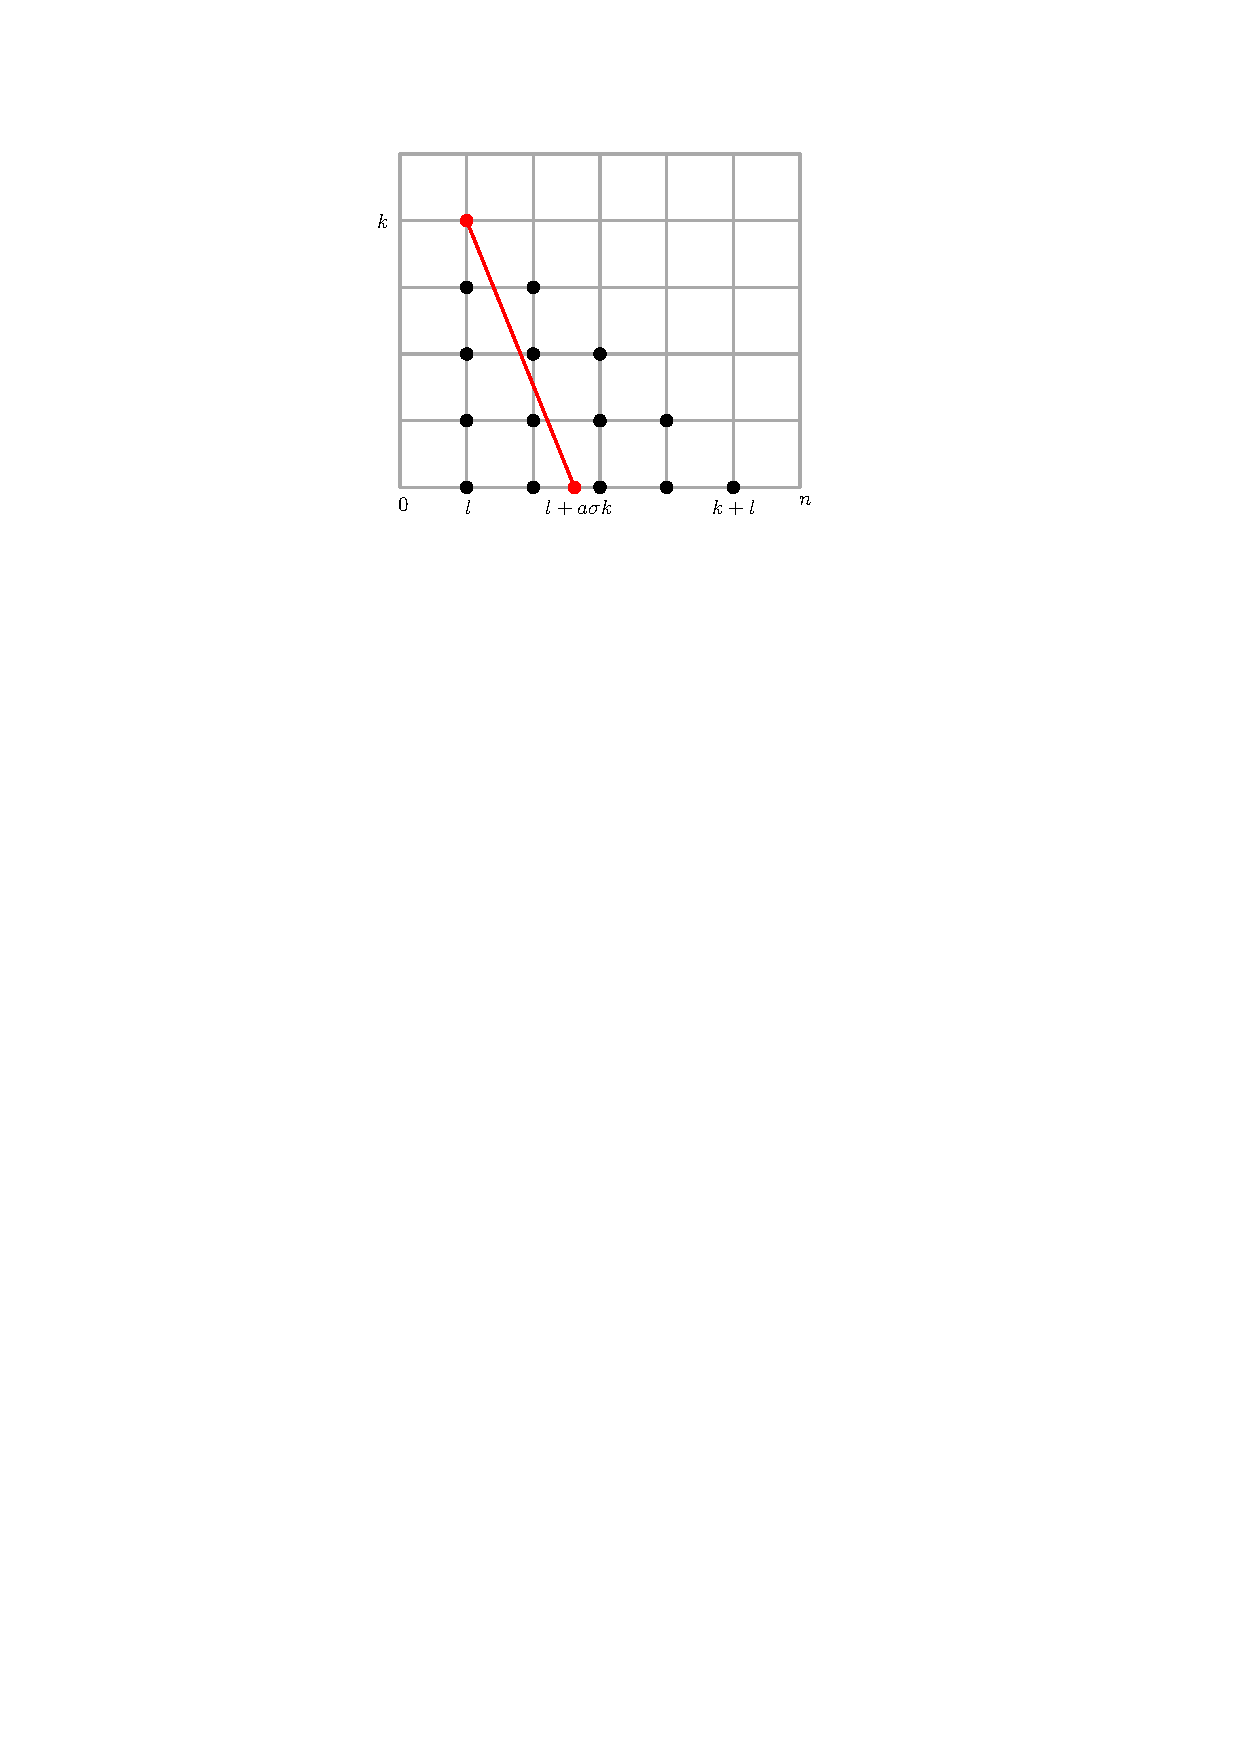
\includegraphics[scale=0.8]{../img/pde/wave-dep.pdf}
        \end{center}
        \caption{К замечанию \ref{rem:wave-dep}.}
    \end{figure}


    \begin{rem}\label{rem:wave-dep}
        Заметим, что $u$ постоянна на прямой $x + at = const$. Будем пока считать $a > 0$. Рассмотрим значение $u_l^k$. Оно должно определятся соответствущим значением на прямой $t = 0$:
        \[
            lh + ak\tau = sh \so s = l + a\sigma k.
        \]
        С другой стороны, в нашей схеме значение $u_l^k$ определяется $u_l^{k-1}$ и $u_{l+1}^{k-1}$. Если продолжить этот процесс до $k = 0$, увидим, что $u_l^k$ зависит лишь от $u^0_l\ldots u^0_{l + k}$. Таким образом, чтобы вообще использовать нужное значение из начальных данных, надо
        \[
            s \leqslant l + k \so l + a \sigma k \leqslant l + k \so a \sigma \leqslant 1.
        \]
        Если $a < 0$, то мы вообще не будем использовать это значение, ибо красная прямая будет наклонена в другую сторону.
    \end{rem}

    Именно с этим связано то, что для $a < 0$ срабатывает схема
    \[
        \dfrac{u^{k + 1}_l - u^k_l}{\tau} = a \dfrac{u^k_{д} - u^k_{l-1}}{h}.
    \]
    В ней информация распространяется в другую сторону, и оценки получаются те же с точностью до знака $a$.

    \paragraph{Схема Куранта-Рисса}

    Рассмотрим теперь систему
    \[
        \dfrac{\pd u}{\pd t} = A \dfrac{\pd u}{\pd x},
    \]
    где $u$~--- вектор из $\R^p$. Будем считать, что $A$~--- симметричная матрица с постоянными коэффициентами (поэтому у неё все собственные числа вещественны).

    Собственные числа матрицы $A$ могут быть разных знаков, это приводит к появлению решений-волн, которые бегут в разные стороны. Это причина, по которой ни одна из простейших схем, вероятно, не будет работать.

    Рассмотрим две матрицы: $A_+$ и $A_-$. Первая из них имеет положительные собственные числа такие же, как у $A$, а вместо отрицательных у неё нули. $A_-$ вместо отрицательных собственных чисел $A$ имеет их модули, а вместо отрицательных~--- нули. 

    \begin{rem}
        Можно эти две матрицы построить в собственном базисе $A$, а потом вернуть их оттуда назад.
    \end{rem}

    В итоге $A = A_+ - A_-$. Схема будет устроена так:
    \[
        \dfrac{u_l^{k+1} - u_l^k}{\tau} = A_+ \dfrac{u^k_{l + 1} - u^k_l}{h}  - A_- \dfrac{u_l^k - u^k_{l-1}}{h}.
    \]
    Естественно ожидать от неё хорошего поведения. Такая схема называется \ti{схемой Куранта-Рисса}. Найдём матрицу перехода; для этого вычислим её на
    \[
        u_l^k = fe^{imx}, \quad f \text{~--- произвольный постоянный вектор.}
    \]
    Такой же подстановкой, как в прошлом пункте, находим
    \[
        c(m) = I + \sigma \left((e^{imh} - 1)A_+ - (1 - e^{-imh}) A_-\right), \quad \sigma = \dfrac{\tau}{h}.
    \]
    Теперь нам надо искать собственные числа <<матрицы>> $C$ (мы тут всё-таки вляпались в многомерие, но не сильно). Запишем условие на собственные числа:
    \[
        g + \sigma \left((e^{imh} - 1)A_+ - (1 - e^{-imh})A_- \right)g = \lambda g.
    \]
    Отсюда
    \[
        \left((e^{imh} - 1)A_+ - (1 - e^{-imh})A_- \right)g = \dfrac{\lambda - 1}{\sigma} g
    \]
    Слева стоит линейная комбинация матриц с известными собственными числами, причём там, где у первой ненулевое собственное число, у второй ноль, и наоборот. Поэтому получаем
    \[
        \lambda = 1 + \sigma \lambda_{A_{\pm}} (e^{\pm imh} - 1).
    \]
    Очень похоже на \ref{eq:wave-trans}, но только теперь $a = \lambda_{A_{\pm}}$ и $m = \pm m$.

    Ясно, что знак $m$ ни на что не повлияет, и теперь $a > 0$. Второе условие получится аналогичным.

    \begin{rem}
        Мы не доказывали достаточность условия для многомерности, но в этом конкретном случае её можно доказать.
    \end{rem}

    \paragraph{Явная схема для уравнения колебаний струны}

    Рассмотрим уравнение колебаний
    \[
        \dfrac{\pd^2 u}{\pd t^2} = \dfrac{\pd^2 u}{\pd x^2}.
    \]

    Вообще, надо было бы перейти к системе уравнений первого порядка, но мы попробуем найти $c(m)$ не переходя~--- вдруг получится!..

    Схема
    \[
        \dfrac{u_l^{k + 1} - 2u_l^k + u_l^{k-1}}{\tau^2} = \dfrac{u^k_{l+1} - 2u^k_l + u^k_{l-1}}{h^2}.
    \]
    Положим
    \[
        u_l^k = e^{imx}, \quad u_l^{k+1} = ce^{imx}, \quad u_l^{k-1} = c^{-1} e^{imx}.
    \]
    Выйдет уравнение на $c$:
    \[
        \dfrac{c + c^{-1}}{2} = 1 + \sigma^2\big(\cos(mh) - 1\big) = p.
    \]
    Решая, получим
    \[
        c = p \pm \sqrt{p^2 - 1}.
    \]
    Неудивительно, что нашлись два значения для каждого $m$: на самом деле это собственные числа матрицы перехода, $\lambda_1$ и $\lambda_2$, потому что система второго порядка!

    Заметим, что по теореме Виета (ну или руками) 
    \[
        \lambda_1 \lambda_2 = 1,
    \]
    поэтому, чтобы была устойчивость, нам нужно, чтобы $|\lambda_1| = |\lambda_2| = 1$. Это условие выполняется, когда корни комплексны:
    \[
        \lambda_{1, \, 2} = p \pm i\sqrt{1 - p^2} \so |\lambda_{1, \, 2}| = 1.
    \]
    Для этого необходимо, чтобы $|p| < 1$. Ещё оно выполняется, когда корни равны. Чтобы они были равны, нужно $p = \pm 1$, поэтому общее условие:
    \[
        |p| \leqslant 1.
    \]

    Посмотрев на формулу для $p$, поймём, что это гарантированно происходит при 
    \[
        \boxed{|\sigma| \leqslant 1}\,.
    \]

    \begin{rem}
        У Ангелины есть ещё много про достаточное условие, у нас этого, к счастью, не было. Можно ещё сказать, что при $\sigma = 1$ на самом деле проявляется слабая неустойчивость, но она не влияет на сходимость.
    \end{rem}

    \paragraph{Явная и неявная схемы для двумерного уравнения теплопроводности}

    \begin{de}
        \ti{Двумерное уравнение теплопроводности}
        \[
            \dfrac{\pd u}{\pd t} = \dfrac{\pd^2 u}{\pd x^2} + \dfrac{\pd^2 u}{\pd y^2}.
        \]
    \end{de}

    Теперь нам понадобится два индекса внизу:
    \[
        u^k_{np} \approx u(nh, \, ph, \, k\tau).
    \]

    Рассмотрим явную схему
    \begin{equation}\label{eq:therm-2-expl}
        \dfrac{u^{k+1}_{np} - u^k_{np}}{\tau} = \dfrac{u^k_{n+1 \; p} - 2u^k_{np} + u^k_{n-1 \; p}}{h^2} + \dfrac{u^k_{n \; p+1} - 2u^k_{np} + u^k_{n \; p - 1}}{h^2}.
    \end{equation}

    Попробуем найти матрицу перехода. Для этого рассмотрим 
    \[
        u^k_{np} = e^{imx} e^{ily}, \quad x = nh, \quad y = ph.
    \]
    Делая стандартную подстановку и преобразования, получаем
    \[
        c(m, \, l) = 1 + 2\sigma\big(cos(mh) - 1\big) + 2\sigma\big(\cos(lh) - 1\big), \quad \sigma = \dfrac{\tau}{h^2}.
    \]
    Чтобы $\big|c(m, \, l)\big| \leqslant 1$ всегда, нужно
    \[
        \boxed{\sigma \leqslant \dfrac{1}{4}}\,.
    \]
    Получилось в два раза жёсткое условие, чем для одномерного уравнения!

    Посмотрим теперь на простейшую неявную схему, в ней левая часть уравнения \ref{eq:therm-2-expl} просто заменится на
    \[
        \dfrac{u^{k}_{np} - u^{k-1}_{np}}{\tau}.
    \]
    Тем же путём находим
    \[ 
        c(m, \, l) = \dfrac{1}{1 - 2\sigma\big(cos(mh) - 1\big) - 2\sigma\big(\cos(lh) - 1\big)}.
    \]
    Видно, что необходимое условие устойчивости выполнено всегда, как и в одномерном случае.

    Поговорим о том, как решать систему уравнений для неявной схемы, которая целиком выглядит вот так:
    \[
        \dfrac{u^{k}_{np} - u^{k-1}_{np}}{\tau} = \dfrac{u^k_{n+1 \; p} - 2u^k_{np} + u^k_{n-1 \; p}}{h^2} + \dfrac{u^k_{n \; p+1} - 2u^k_{np} + u^k_{n \; p - 1}}{h^2}.
    \]
    Если её переписать, выйдет
    \[
        (1 + 4\sigma) v_{np} - \sigma v_{n + 1\; p} - \sigma v_{n \; p+1} - \sigma v_{n - 1\; p} - \sigma v_{n \; p-1} = \alpha_{np},
    \]
    где
    \[
        v_{np} = u_{np}^k \text{ и } \alpha_{np} = u^{k-1}_{np}.
    \]
    Граничные условия, как обычно в последнее время, I типа:
    \[
        v_{00} = v_{0N} = v_{N0} = v_{NN} = 0.
    \]
    Поэтому будем рассматривать $n$ и $p$ от $1$ до $N-1$. 

    Упорядочим элементы $v$ следующим образом:
    \[
        v_{11}, \; v_{12}, \; \ldots, \; v_{1 \; N-1}, \; v_{21}, \; \ldots
    \]
    Тогда матрица системы (для примера $N=4$) будет выглядеть так:
    \[
        \begin{array}{ccc|ccc|ccc}
        1 + 4\sigma & -\sigma & 0 & -\sigma & 0 & 0 & 0 & 0 & 0 \\
        -\sigma & 1 + 4\sigma & -\sigma & 0 & -\sigma & 0 & 0 & 0 & 0 \\
        0 & -\sigma & 1 + 4\sigma & 0 & 0 & -\sigma & 0 & 0 & 0 \\
        \hline
        -\sigma & 0 & 0 & 1 + 4\sigma & -\sigma & 0 & -\sigma & 0 & 0 \\
        0 & -\sigma & 0 & -\sigma & 1 + 4\sigma & -\sigma & 0 & -\sigma & 0 \\
        0 & 0 & -\sigma & 0 & -\sigma & 1 + 4\sigma & 0 & 0 & -\sigma \\
        \hline
        0 & 0 & 0 & -\sigma & 0 & 0 & 1 + 4\sigma & -\sigma & 0 \\
        0 & 0 & 0 & 0 & -\sigma & 0 &  -\sigma & 1 + 4\sigma & -\sigma \\
        0 & 0 & 0 & 0 & 0 & -\sigma & 0 & -\sigma & 1 + 4\sigma
        \end{array}
    \]
    В общем случае получается $(2N-1)$-диагональная матрица.

    Пусть
    \[
        v_n = (v_{n1}, \, \ldots, \, v_{n \; N-1}), \quad \alpha_n = (\alpha_{n1}, \, \ldots, \, \alpha_{n \; N-1}).
    \]
    Тогда можно записать систему, как
    \[
        A_n v_{n-1} + B_n v_n + C_n v_{n+1} = \alpha_{n},
    \]
    где $A_n, \; B_n$ и $C_n$~--- блоки из соответствующей строки.
    Дальше можно действовать так же, как обычной прогонкой. Это называется \ti{матричная прогонка}.

    К сожалению, обычная прогонка содержит умножения чисел, которые делаются за $O(1)$, и работает $O(N)$, а матричная прогонка содержит умножения матриц, которые делаются за $O(N^3)$, и работает за $O(N^4)$. Долго! Поэтому нам такой неявный метод не подходит.

    \paragraph{Схема продольно-поперечной прогонки}

    Нужно сделать систему трёхдиагональной. Естественное желание~--- вынести часть переменных в правой части уравнения на соседний слой, чтобы сократить количество тех, что входит с текущего. Эта идея приводит к схеме

    \[
        \dfrac{u^{k+1}_{np} - u^{k}_{np}}{\tau} = \dfrac{u^{k+1}_{n+1 \; p} - 2u^{k+1}_{np} + u^{k+1}_{n-1 \; p}}{h^2} + \dfrac{u^k_{n \; p+1} - 2u^k_{np} + u^k_{n \; p - 1}}{h^2}.
    \]
    Если переписать, получится
    \[
        \sigma u^{k+1}_{n-1 \; p} - (1 + 2\sigma) u_{np}^{k+1} + \sigma u^{k+1}_{n+1 \; p} = \alpha_{np}.
    \]
    Матрица трёхдиагональная, всё замечательно.

    Надо проверить на устойчивость. Обычной техникой получаем
    \[
        c(l, \, m) = \dfrac{1 - 2\sigma(1 - \cos lh)}{1 + 2\sigma(1 - \cos mh)}.
    \]
    Чтобы эта штука всегдя была меньше $1$ по модулю, нужно
    \[
        \boxed{\sigma \leqslant \dfrac{1}{2}}\,.
    \]
    Только условная устойчивость!

    Можно рассмотреть аналогичную схему
    \[
        \dfrac{u^{k+1}_{np} - u^{k}_{np}}{\tau} = \dfrac{u^{k}_{n+1 \; p} - 2u^{k}_{np} + u^{k}_{n-1 \; p}}{h^2} + \dfrac{u^{k+1}_{n \; p+1} - 2u^{k+1}_{np} + u^{k+1}_{n \; p - 1}}{h^2}.
    \]
    У неё свойства примерно такие же, только $l$ и $m$ меняются местами.

    Идея: чередовать схемы I и II:
    \[
        2k \xrightarrow{\text{I}} 2k+1 \quad 2k+1 \xrightarrow{\text{II}} 2k+2.
    \]
    Пусть у чётных слоёв будет номер $k$, у нечётных~--- $k + \nicefrac{1}{2}$. Ну и просто пишем последовательно формулы для I сначала, потом для II, и получаем переход
    \[
        k \to k+ \frac{1}{2} \to k+1.
    \]

    Ясно, что при этом коэффициенты перехода перемножатся:
    \[
        C = C_{\text{I}} C_{\text{II}} = \dfrac{1 - 2\sigma(1 - \cos lh)}{1 + 2\sigma(1 - \cos mh)} \cdot \dfrac{1 - 2\sigma(1 - \cos mh)}{1 + 2\sigma(1 - \cos lh)}.
    \]
    У этой штуки получается $|c| \leqslant 1$ всегда, наступает абсолютная устойчивость.

    Такую схему называют \ti{схемой продольно-поперечной прогонки.}

    \begin{rem}
        К сожалению, если то же самое сделать для трёхмерного уравнения теплопроводности (а там будет три схемы и разбиение слоя на три подслоя), абсолютной устойчивости не выйдет. Это можно проверить прямым вычислением.
    \end{rem}

    \begin{rem}
        Более подробно все выкладки можно прочитать у Ангелины, там всё понятно. Ещё там рассказывается про \ti{схему расщепления}, которая всегда работает. Потом есть разговоры про то, как избавиться от наших общих ограничений вроде периодичности граничных условий, кубической формы области и постоянных коэффициентов.
    \end{rem}







\end{document}
